% !TeX root = ../../main.tex
\section{Experiments}\label{section:experiments}

Three main experiments were implemented to demonstrate how the smartphone can help with common interactions when using \ac{VR} software.
To achieve consistency amongst all experiments in terms of look and basic functionality, a parent class was implemented. The parent class implements utilities, which are required by each experiment. It also sets up a basic scene, which contains a sky, a floor and lights. Also the connection to the \ac{UBII} server is handled. 


\subsection{Model Viewer}\label{subsection:model-viewer}

\acl{VR} offers a new way of experiencing \ac{3D} content. It is more convenient to view a model from different angles and gives a feel of a real presence of the object. Model viewers like Sketchfab\footnote{Sketchfab is an online platform to publish and view \ac{3D} content. Website: \href{https://sketchfab.com}{www.sketchfab.com}} have implemented \ac{VR} support a while ago~\cite{Denoyel.2016}. But this experience can be enhanced with a smartphone. Models can be rotated without changing the position of the headset or using s expensive hand motion tracking system.

\citeauthor{Katzakis.2010} implemented this without \ac{VR}. His approach uses a smartphone to rotate a model which is displayed on a conventional display. He uses a similar setup, in which the phone is wireless connected to a computer where the model is rendered. The orientation data comes from the magnetometer and, once calibrated to the screen position, is directly mapped to the model~\cite[139]{Katzakis.2010}. In the evaluation of a mouse, a touch pen and the smartphone, the latter wins in terms of the time it takes to rotate the model to a certain pose~\cite[140]{Katzakis.2010}. 
Since this approach turned out to be very successful, it was used in this experiment as well. 

To feature how easy it is to view a more complex model using VR and the smartphone as a manipulator, a human skeleton model is used. This experiment is the only one supporting more than one smartphone client at the same time. For every client that connects, a new skeleton is created. The position is fixed and arranged around the position of the \ac{VR} headset. A scene with multiple connected clients is shown in Figure~\ref{fig:screenshot-exp-mv}.

\begin{figure}[htpb]
  \centering
  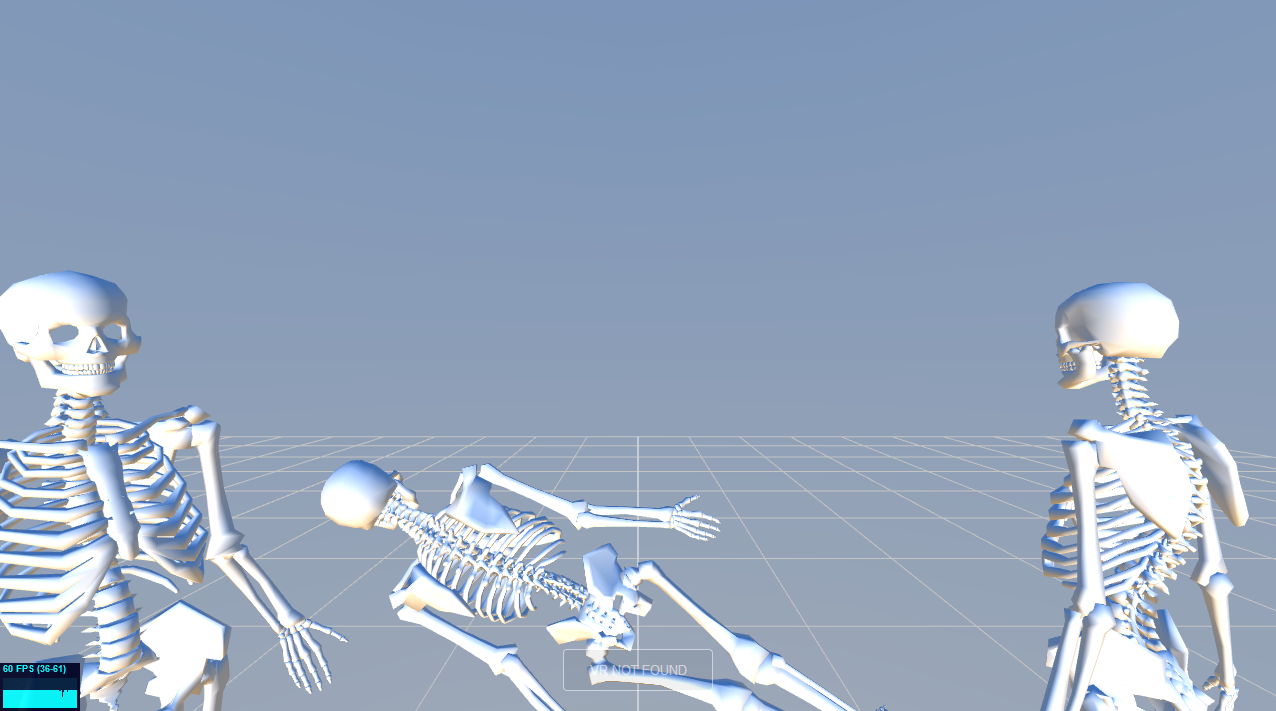
\includegraphics[width=12cm]{figures/screenshot_exp_mv.png}
  \caption[Screenshot of the model viewer experiment]{A screenshot of three devices being connected and controlling the rotation of the models.}\label{fig:screenshot-exp-mv}
\end{figure}

% Note: latex thinks the hbox is overfull. This is not the case because something is fixing it. Try removing all words after the lstinline, then you will see that it overflows. But when using in an sentence it appears to be rescaled.
The implementation of this experiment listens for new clients. As soon as one connects, a new \ac{UBII} interaction is published and the resulting \ac{UBII} topic subscribed. Since the smart device (see Section~\ref{section:smart-device}) publishes the orientation data in a different format than ThreeJS needs for rendering, a reusable \ac{UBII} interaction was created. The \ac{UBII} interaction converts the angles from radian to degrees, changes the coordinate system and publishes them to the \lstinline[breaklines=false]{[client id]/SAVRLaserPointer/orientation} topic. The code for the \ac{UBII} interaction is shown in Figure~\ref{fig:ubii-interaction-angles}.

\begin{figure}[H]
  \begin{lstlisting}[language=JavaScript]
    function (input, output, state) {
      if (!input) {
        return;
      }

      const deg2Rad = function(v) {
        return v * Math.PI / 180;
      };

      output.orientation = {
        x: deg2Rad(input.orientation.y),
        y: deg2Rad(input.orientation.x),
        z: deg2Rad(-input.orientation.z)
      };
    }
  \end{lstlisting}
  \caption[UBII interaction converting euler angles in radians to degrees]{This \ac{UBII} interaction is used to convert the orientation data sent by the smart device to the format ThreeJS needs for rendering. The values are converted by multiplying with an approximate of the number $\Pi$ (\enquote{PI}) and dividing by $180$.}\label{fig:ubii-interaction-angles} %chktex 46
\end{figure}


\subsection{Laser Pointer}\label{subsection:laser-pointer}

Selecting elements in a virtual world is a basic interaction most \ac{VR} applications use. The selection of elements in a \ac{2D} environment with standard input devices like a mouse or touch screen is trivial. But the selection of elements in a \ac{3D} environment is problematic, because the element might be too far away from the the user or the cursor. Ray casting\footnote{Ray casting describes a technique to determine the objects which intersect with a ray, cast from a given point into a given direction.} is used to solve this problem: A ray, with the tracked device as origin, is created. Then, the element first hit by the ray is selected. Implementations without a tracked device, often use the position and orientation of the headset. The ray is fixed to the head of the user and casted along his viewing direction~\cite[23]{Kamm.2018}. This forces the user to keep the head still and look at a certain object to select it, until a button is pressed or a certain time has passed.

% TODO: maybe explain some more strategies, like in the keyboard chapter

A better solution is the use of handheld controllers, where the position of the controller is used as origin for the ray. Since the smartphone provides orientation data, it can be used for this task, too. But most handheld controllers have also positional tracking, which allows them to represent the hand of a user by displaying a virtual phone. This emulates the use of a handheld laser pointer in the real world. Since a smartphone does not have positional tracking, the origin has to be somewhere else. Again, the head could be used, but then the user would have no visual representation of the rotation of the phone. To give the user a better feel for direction he is pointing, a visual representation is needed. The user has to see where the ray is going, even when rotating it in the opposite direction of the view direction.

\citeauthor{Argelaguet.2013} evaluated more than 30 different selection techniques for virtual environments, but there are no technique that uses the orientation but not the position of the pointing device~\cite[Table 1]{Argelaguet.2013}. To work around the missing position data of the device, the ray origin is set to a fixed location relative to the users head where the phone could be in the real world. The ray origin is represented by a \ac{3D} phone model, which orientation is synchronized with the one from the last connected smart device (see Section~\ref{section:smart-device}) client, similar to the first experiment (\ref{subsection:model-viewer}). To keep the virtual phone inside the view frustum of the user, it rotates relative to the user on the \(y\)-axis.
A line is attached to the front of the phone (the \enquote{laser}) to indicate the direction of the ray.

\begin{figure}[htpb]
  \centering
  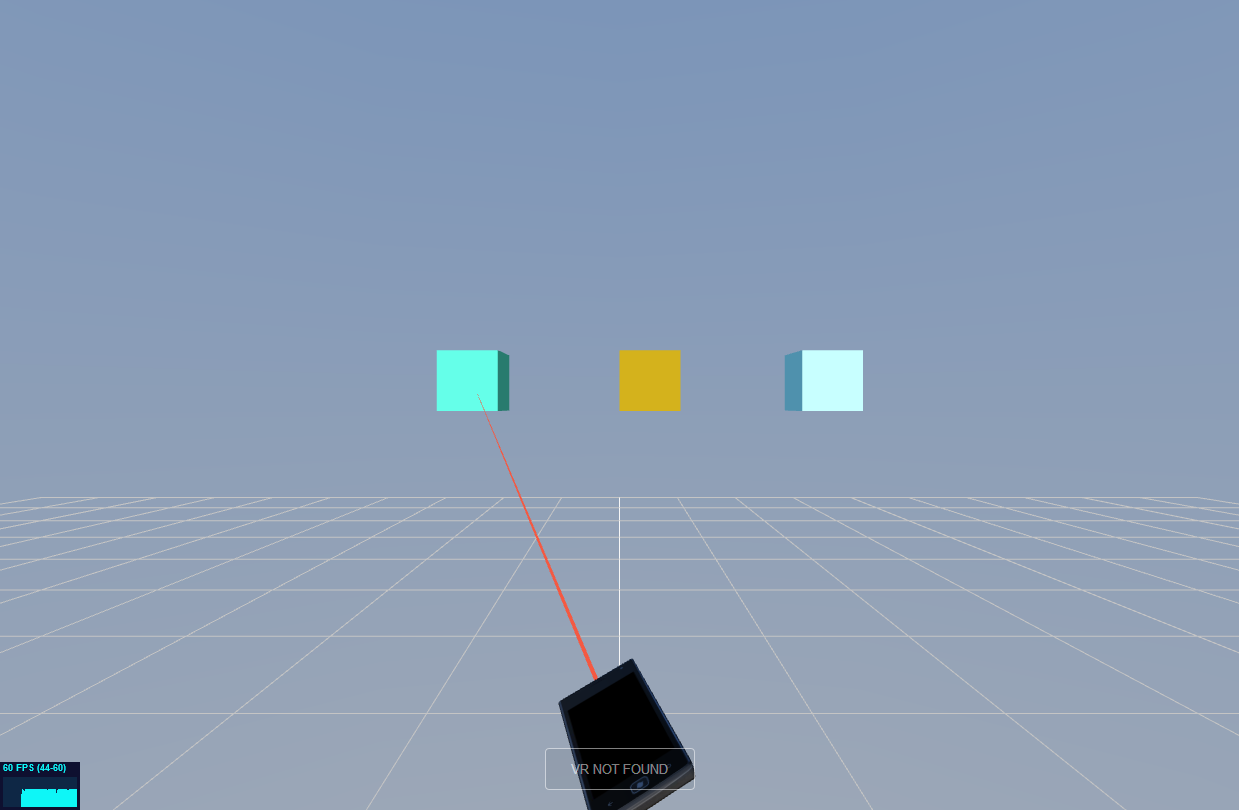
\includegraphics[width=12cm]{figures/screenshot_exp_lp.png}
  \caption[Screenshot of the laser pointer experiment]{A screenshot of the virtual laser pointer and selectable cubes.}\label{fig:screenshot-exp-lp}
\end{figure}

In addition to the orientation \ac{UBII} topic, this implementation subscribes to the touch events topic. The touch down event is needed to trigger the actual selection.
In this experiment cubes float in front of the user. If he points the laser at one and touches the display, the cube will change it's color. This works not only with cubes, but with any mesh. Also the system can trigger any kind of event or action. A screenshot of this setup can be seen in Figure~\ref{fig:screenshot-exp-lp}.


\subsection{Virtual Keyboard}\label{subsection:virtual-keyboard}

Text input is not an easy task to perform in \ac{VR}. But it is often required for labeling, annotation, entering filenames for saving operations and setting parameters in visualizations and other productive \ac{VR} software~\cite[2154]{Rhoton.2002}. This is why a lot of applications try to avoid it. 

Tilt Brush\footnote{Tilt Brush by Google is a tool for three-dimensional painting in VR. Website: \href{https://www.tiltbrush.com/}{www.tiltbrush.com}} solves this by identifying their scenes with a screenshot of the scene rather than a filename. To save a scene, the users gets a virtual camera attached to his hand motion controller, which he then uses to make a thumbnail of the current scene~\cite{GoogleLLC.2019}. % chktex 13
Others use a laser pointer either attached to a hand controller or to the headset to select keys on a \ac{2D} image of a keyboard~\cite{WeelcoInc.2017}. A more recent approach is the frequently called \enquote{drum keyboard}, which attaches drum sticks to the hand controllers which are then used to hit the keys~\cite{Weisel.2017}. 
There are also approaches which do not use hand controllers, like hand gloves~\cite{Evans.1999,Rhoton.2002}, a real keyboard~\cite{McGill.2015,Walker.2017} or other peripherals~\cite[111\psq]{Gonzalez.2009}. Other experimental methods are speech recognition~\cite[2154\psqq]{Rhoton.2002} and handwritten character recognition~\cite[113]{Gonzalez.2009}.

Similar to the approach by~\citeauthor{Dias.2018} to implement user interfaces using a real smartphone and a virtual representation visible in the \ac{VR} headset~\cite[5]{Dias.2018}, this experiment displays a virtual keyboard in \ac{VR} as seen in Figure~\ref{fig:screenshot-exp-vk}. 
The surface of the virtual keyboard is mapped to the touchscreen of the smart device (see Section~\ref{section:smart-device}). The cursor, represented by a blue circle, visualizes the position of the finger on the touchscreen. The cursor is only visible when the smartphone sends touch position data, which is only the case when the user is touching the screen. To select a key, the user has to move the cursor on top of a key and then keep the finger there for roughly a second. As long as the user is holding his finger on a key to select it, the blue circle fills up with another circle to indicate the running selection progress. When executing the key press on the first touch and without a cursor, the user would not know which key he is going to hit with his finger, because his sight is obscured by the \ac{VR} headset. \citeauthor{Dias.2018} work around this problem by using a Leap Motion sensor to visualize the finger positions~\cite[4]{Dias.2018}.

\begin{figure}[H]
  \centering
  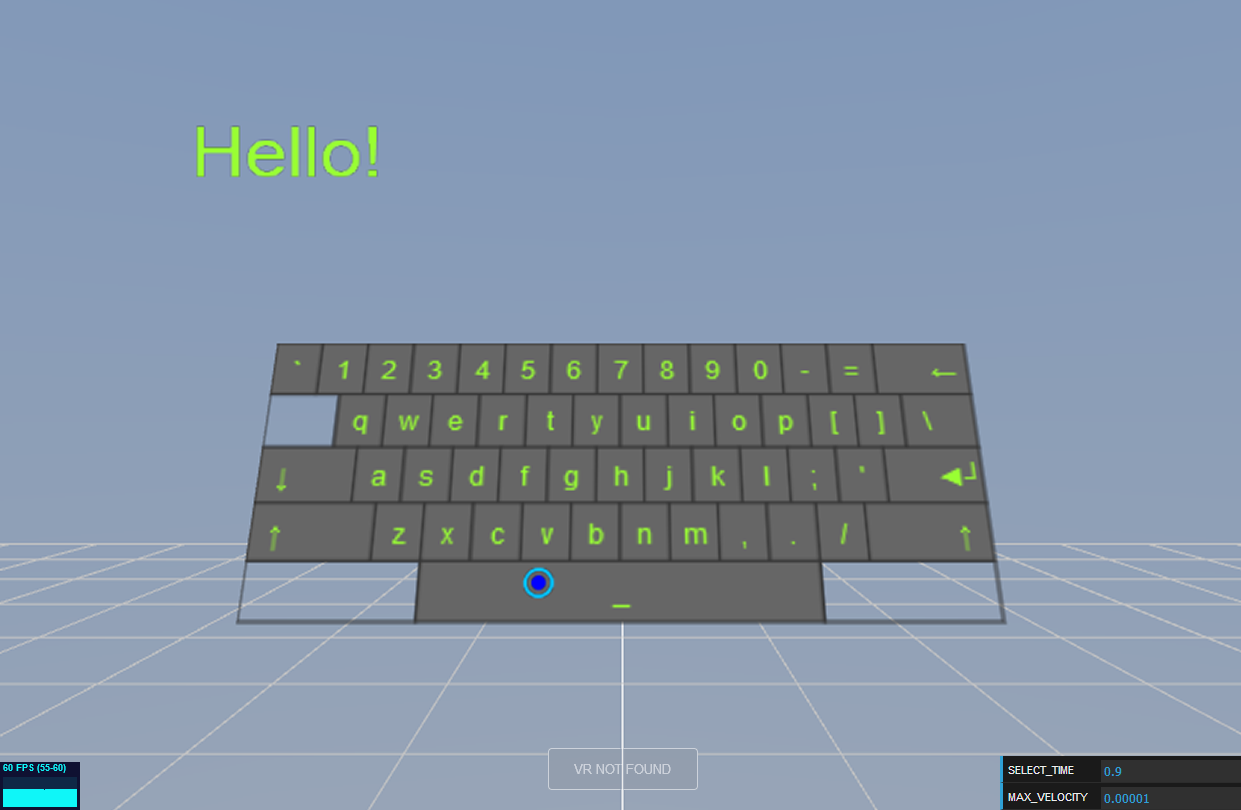
\includegraphics[width=12cm]{figures/screenshot_exp_vk.png}
  \caption[Screenshot of the virtual keyboard experiment]{A screenshot of the virtual keyboard with the blue cursor and the previously typed text.}\label{fig:screenshot-exp-vk}
\end{figure}

Three components were implemented as \acl{JS} classes for this experiment. The \lstinline{SmartphoneCursor} component uses the touch events and position data to display a blue circle (the cursor) on a given area in the scene. The cursor is only shown, when the touch screen is pressed. If it is pressed, the position of the circle is synchronized with the position of the finger on the touch screen. To detect intentional movements, the current position (vector) is subtracted by the position (vector) of the previous frame. If the length of the resulting vector is smaller than a certain threshold value, it is assumed that this was not an intended movement. This calculation depends on the current framerate, which is not a good practice because the threshold value will behave differently depending on the current framerate. But as the target framerate is 60 frames per second and the testing system does not have issues in reaching this target, it is not a critical problem.
As long as intentional movements are not detected, a timer counts up to a certain value (with the default settings, roughly one second). After this, the counter and a select event containing the cursor position is sent to the main program. To visualize this, a second blue circle gets larger until it fills up the whole cursor and finally disappear again. 

The second component renders a virtual QWERTY\footnote{The name QWERTY describes the US layout for computer keyboards.} keyboard to the scene. The keyboard layout can be changed pretty easily as shown in Figure~\ref{fig:virtual-keyboard-layout}. Every key has a character or an action assigned as well as properties which influence the look. Special keys like the caps, caps lock, enter and delete key are fully functional as known from a real keyboard. If caps lock is activated, the key is drawn in blue and all characters are display in upper case. The \lstinline{VirtualKeyboard} class draws the keyboard with just the keyboard layout, a height and a width as input. If the \lstinline{onPress(coordinates)} function is called, for example by the cursor component, the pressed key is calculated and returned using the provided position. The main program then applies the key to a string and sends the result to the third component. % chktex 36

\begin{figure}[H]
  \begin{lstlisting}[language=JavaScript]
  // rows
  [
    // columns
    %\dots%
    [ 
      // keys
      %\dots%
      {
        key: '=',                             // the returned character if no action is present otherwise just a label
        keyCaps: '+'                          // the returned character if in caps mode 
      },
      {
        key: '%\color{TUMAccentOrange}\textleftarrow%',
        action: KEY_ACTIONS.DELETE_ONE,       // a special key action; in this case, it deletes the last character
        width: 2,                             // with of the key
        align: KEY_ALIGNMENT.RIGHT            // the alignment of the label on the key
      }
      %\dots%
    ],
    %\dots%
  ],
  \end{lstlisting}
  \caption[Virtual keyboard layout definition]{The definition of the virtual keyboard layout in \ac{JS}. It is defined as a \ac{2D} array, where the first dimension corresponds to the key rows and the second one to the keys column wise.}\label{fig:virtual-keyboard-layout}
\end{figure}

The \lstinline{TextDisplay} component just renders a given text inside a given area to a texture. If the text is changed it automatically updates and redraws the texture.